% ex: ts=2 sw=2 sts=2 et filetype=tex
% SPDX-License-Identifier: CC-BY-SA-4.0

\documentclass{article}
\usepackage[utf8]{inputenc}
\usepackage{geometry}
 \geometry{
 letterpaper,
 total={170mm,257mm},
 left=20mm,
 top=20mm,
 }
 \usepackage{graphicx}
 \usepackage{titling}

 \title{Escándalo Schön}
\author{Yolanda Alejo Huerta}
\date{Septiembre 2025}
 
 \usepackage{fancyhdr}
\fancypagestyle{plain}{%  the preset of fancyhdr 
    \fancyhf{} % clear all header and footer fields
    \fancyfoot[R]{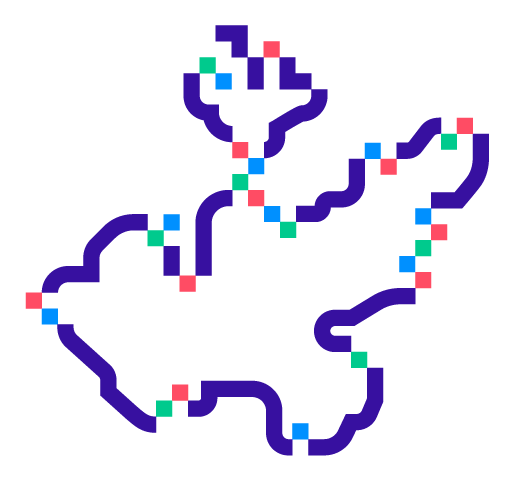
\includegraphics{tsj_jalisco.png}}
    \fancyfoot[L]{\thedate}
    \fancyhead[L]{Escándalo Shön}
    \fancyhead[R]{\theauthor}
}
\makeatletter
\def\@maketitle{%
  \newpage
  \null
  \vskip 1em%
  \begin{center}%
  \let \footnote \thanks
    {\LARGE \@title \par}%
    \vskip 1em%
    %{\large \@date}%
  \end{center}%
  \par
  \vskip 1em}
\makeatother

\usepackage{lipsum}  
\usepackage{cmbright}

\begin{document}

\maketitle

\noindent\begin{tabular}{@{}ll}
	Alumna & \theauthor\\
	Profesor & Dr. Paulo Lopez Meyer
\end{tabular}

\section*{Descripción General}
El caso de \textbf{Jan Hendrik Schön} fue uno de los \textbf{mayores
escándalos de fraude científico} en la historia reciente. Ocurrió a principios de la década de 2000 y se centró en un físico que trabajaba en los Laboratorios Bell.

\section*{Resumen del caso}

Jan Hendrik Schön era un prometedor joven físico alemán que, en un corto
período, publicó una serie de \textbf{artículos revolucionarios} sobre
semiconductores y superconductores moleculares en revistas de alto prestigio
como Science y Nature. Sus descubrimientos, que incluían la creación de
transistores moleculares que eran más pequeños y eficientes que los
tradicionales, generaron un enorme interés en la comunidad científica.


Sin embargo, otros científicos comenzaron a notar \textbf{inconsistencias
en sus datos}. Algunos de los gráficos y mediciones en diferentes artículos, que
supuestamente provenían de experimentos distintos, eran
\textbf{sorprendentemente idénticos}. Esto levantó sospechas de que los
datos no eran resultados genuinos de experimentos, sino que habían
sido fabricados.


Una investigación interna de los Laboratorios Bell confirmó que Schön había
\textbf{falsificado y manipulado una gran cantidad de datos}. Se descubrió que
simplemente había copiado y pegado gráficos, y que sus resultados no podían
ser replicados por otros laboratorios. La investigación concluyó que los
hallazgos de Schön eran fraudulentos.

Como resultado, \textbf{más de 20 de sus artículos fueron retractados}, un
número sin precedentes en la ciencia moderna. La Universidad de Constanza en
Alemania, donde había obtenido su doctorado, le retiró su título. Este caso
no solo desacreditó a Schön, sino que también provocó un debate a nivel
mundial sobre la integridad de la investigación, el proceso de revisión por
pares y la presión por publicar en el mundo académico.

\section*{Ejemplo de los artículos fraudulentos}

Los artículos retractados se publicaron en revistas como \textbf{Nature}
y \textbf{Science}, y algunos de los más notables incluyen:

\begin{itemize}
  \item "A gate-induced superconducting state in organic single crystals" (Nature, 2001)
  \item "Superconductivity in molecular crystals induced by charge injection" (Science, 2001)
  \item "Field-effect modulation of the conductance of single molecules" (Nature, 2001)
  \item "High-mobility organic field-effect transistors with a controlled grain boundary density" (Nature, 2001)
\end{itemize}

El factor común en estos y otros trabajos retractados era que los datos
presentados eran idénticos o repetidos, a pesar de que los experimentos
descritos eran supuestamente distintos. Esta fue la pista principal que
alertó a la comunidad científica y condujo a la investigación que descubrió
la fabricación de los datos.

\end{document}
